\section{Preliminary design and evaluation}

This section presents some preliminary design choices that potentially address some of the key challenges (see Section~\ref{sec:video}) in building a traffic map by video measurement. In particular, we focus on

\begin{packeditemize}
	\item Attributing end-to-end performance to link-level knowledge via bottleneck identification.
	\item Identifying unavailable server IP and path information via extrapolating IP and path information from known data.
\end{packeditemize}

For each technique, we will first clarify the assumption, then present the methodology and finally use trace-driven approach to valide the feasibility.

\begin{figure}[h]
\begin{center}
%\includegraphics[]{p1_2Fig.ps}
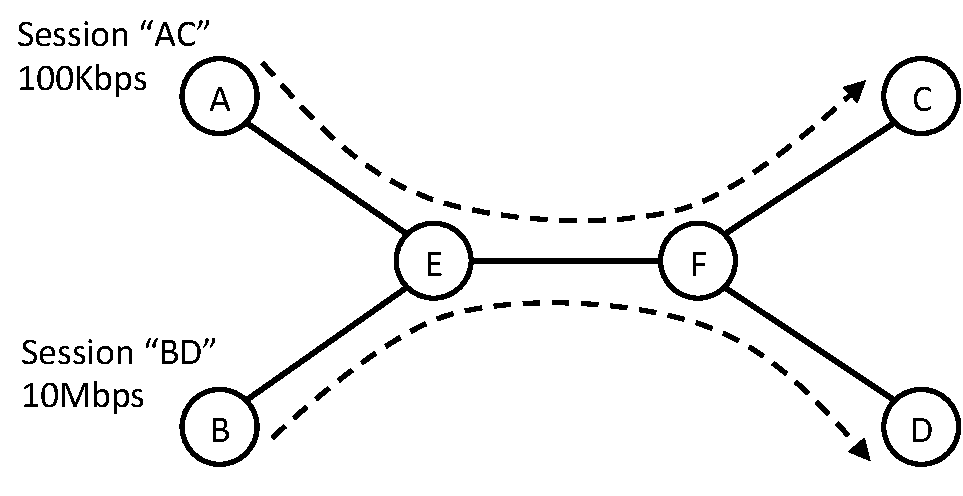
\includegraphics[scale=0.4] {figures/bottleneckExample.pdf}
\caption{Simple example of bottleneck inference algorithm.}
\label{fig:idea:example}
\end{center}
\end{figure}

\subsection{Attributing paths to links}
\begin{packeditemize}
	\item It is used in step 3 in backend processing. The goal is to find infer the available bandwidth on each link from the measured bandwidth of all paths we collect.
	\item Two assumptions (i) the path available bandwidth is determined by the bottleneck link, and (ii) any other link on the path will have larger available bandwidth. Therefore, the goal is identical to identifying the bottleneck link of a path and attribute the path bandwidth to the bottleneck link.
	\item Based on (ii), we develop the ``bottleneck inference algorithm'' as follows...
	\item Real data validation:
		\begin{packeditemize}
			\item Simulation setup: real topology, simulated path performance
			\item Results
		\end{packeditemize}
\end{packeditemize}

\begin{figure}[h]
\begin{center}
%\includegraphics[]{p1_2Fig.ps}
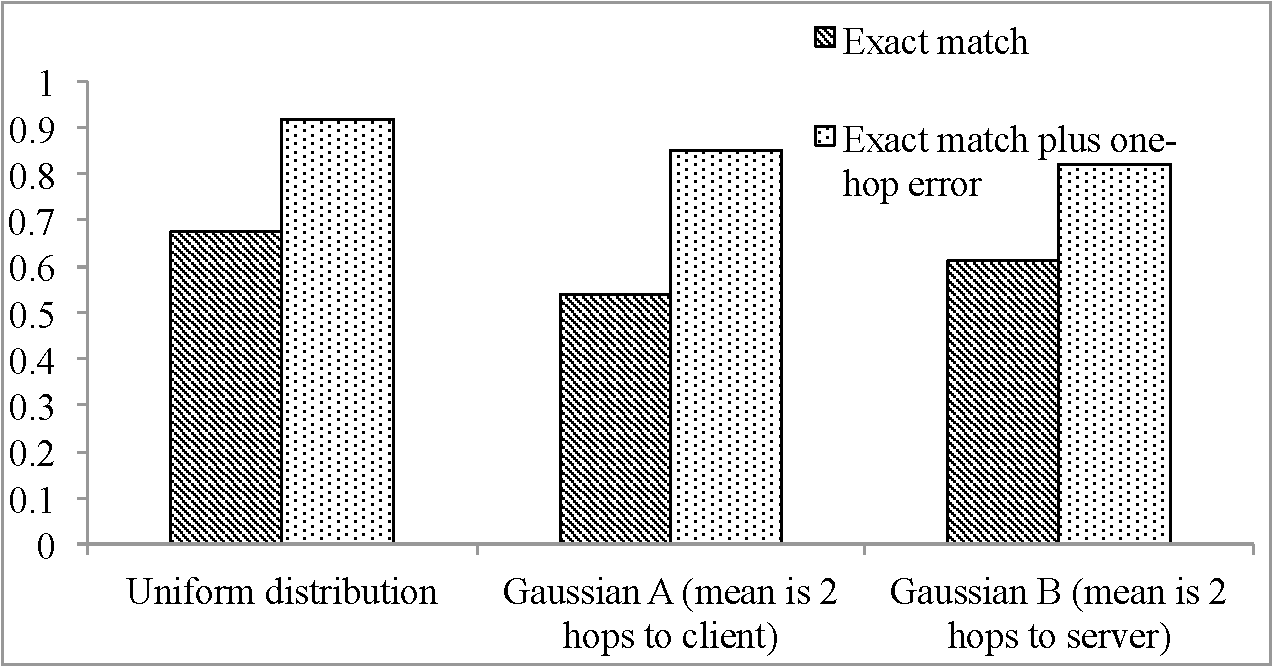
\includegraphics[scale=0.4] {figures/bottle-sim-bar.pdf}
\caption{Simulation-based validation for bottleneck inference technique under three bottleneck distributions. Y: the accuracy in identifying the bottleneck.}
\label{fig:idea:simulation1}
\end{center}
\end{figure}

\subsection{Extrapolate server AS}
Many player only provides the CDN name where the server is located rather than the server AS. To make the best use of all measured video sessions, our goal is to extrapolate the server AS for sessions with CDN name using other sessions of the same CDN.
\begin{packeditemize}
	\item It is used in step 1 in backend processing. We assume that CDNs have a few number of centralized server clusters (Level3, limelight) or a relative static redirecting framework.
	\item Introduce the technique.
	\item Validation in real data (from old results)
\end{packeditemize}

